% ----------------------------------------------------------------------
\begin{frame}[shrink]%[allowframebreaks]
  \frametitle{Spatially-extended systems : \cGL}

  % \begin{figure}[ht]
  \begin{center}
    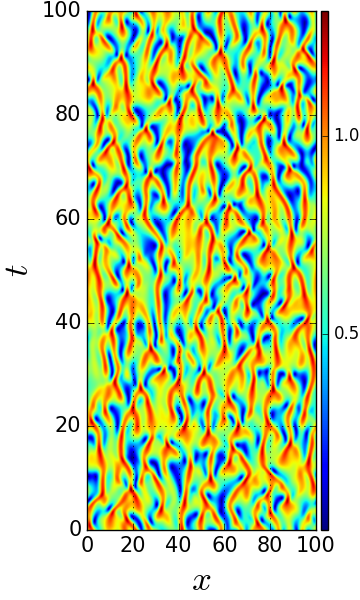
\includegraphics[height=0.6\textheight]{cGL_L100N256}
    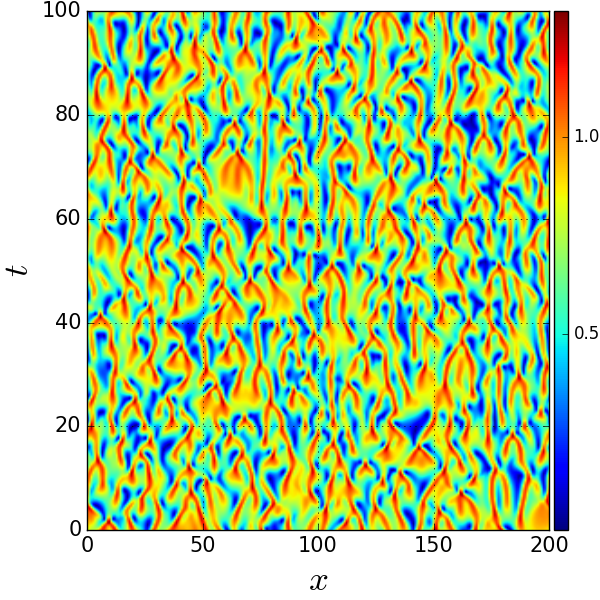
\includegraphics[height=0.6\textheight]{cGL_L200N256}

    {
      $A_t = A + (1 + i\alpha)A_{xx} - (1 +i\beta)|A|^2A$\,,\;
      $\alpha=2$ and $\beta=-2$.
    }
    % \label{fig:cGL_LargeL}
  \end{center}

  \vfill
  \htbc{\scriptsize
    Recurrent patterns not only show up along the \htr{temporal axis}
    \\
    but also along the \htr{spatial axis}
  }
\end{frame}

% ----------------------------------------------------------------------
\begin{frame}%[shrink]
  \frametitle{\small Localized solutions : \cqcGLe}
  {\small
    Following the localized solutions theory of transitional turbulence
    on large domains\footfullcite{BaGuGr16}, here
    I focus on dissipative \emph{\color{blue} soliton} solutions
  }

  {\centering
    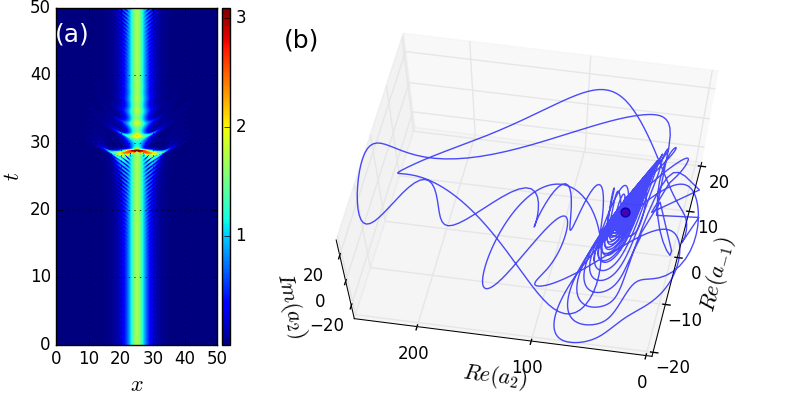
\includegraphics[height=0.6\textheight]{cqcgl_req_explosion}

    $A_t = \mu A + (D_r + iD_i)A_{xx} + (\beta_r + i\beta_i)|A|^2A
    + (\gamma_r + i\gamma_i)|A|^4A
    $
  \par}

\end{frame}

% ----------------------------------------------------------------------
\begin{frame}[shrink]
  \frametitle{Discovery : exploding \rpo\ phase}
  {\small
    A new class of \emph{\color{blue} exploding solitons} !
  }
  {\centering
    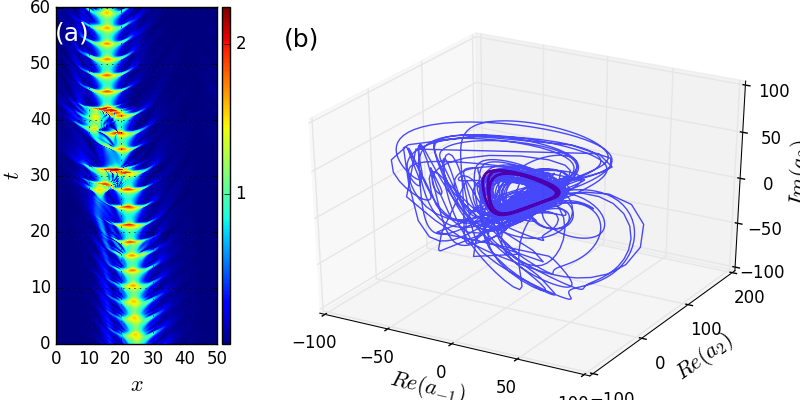
\includegraphics[height=0.5\textheight]{cqcgl_rpo_explosion}
    \par}
  Two completed papers :
  \setbeamercolor{block title}{fg=white, bg=green!75!black}
  \begin{block}{}
    \textrm{
      \small
      % X. Ding  and P. Cvitanovi\'c,
      ``Relative periodic orbit explosion in cubic-quintic complex
      {Ginzburg--Landau} equation''\rf{DingCvit16}
    }
  \end{block}
  \setbeamercolor{block title}{fg=white, bg=green!75!black}
  \begin{block}{}
    \textrm{
      \small
      % X. Ding  and , P. Cvitanovi{\'c} and S. H. Kang,
      ``Integration of a cubic-quintic complex {Ginzburg--Landau} exploding
      soliton''\rf{DingKang16}
    }
  \end{block}
  but no time to discuss this here

\end{frame}
